% !Mode:: "TeX:UTF-8"
% VL 9, gebaut aus part-representation-learning/15-variational-autoencoder.md,
% 16-word2vec.md und 17-representation-learning-graphen.md
% (Dialogmuster: transcripts/vl08-vae-word2vec-2025 und vl09-representation-learning-2025).
% !Mode:: "TeX:UTF-8"
\newcommand{\thepage}{} % to silence a hyperref warning about pdfpagelabels
\RequirePackage[]{silence}
\WarningsOff[hyperref]
\PassOptionsToPackage{log-declarations=false}{xparse}
%\RequirePackage[l2tabu, orthodox]{nag}
\RequirePackage{luatex85} % to make \pdf...= commands work with LuaTeX
\documentclass[aspectratio=169,t]{beamer}
\usepackage{ifthen}
\usepackage[T1]{fontenc}
\usepackage{iftex}
\ifLuaTeX
 \usepackage{fontspec}
 \setmainfont[Ligatures=TeX]{Source Sans Pro}
\else
 \usepackage[utf8]{inputenc}
\fi
\usepackage{german}
\usepackage{newunicodechar}
\newunicodechar{€}{\texteuro}
\newunicodechar{ß}{\ss}
\renewcommand{\SS}{\iffontchar\font"1E9E \symbol{"1E9E}\else SS\fi}
\usepackage{ellipsis}
\usepackage{microtype}
\usepackage{listings}
\usepackage{sourcecodepro}
\lstset{language=Python, basicstyle=\ttfamily}
\usepackage{amsfonts}
\usepackage{amssymb}
\usepackage{amsthm}
\usepackage{fancyhdr}
\usepackage{graphicx}

\newtheorem{proposition}[theorem]{Proposition}

\DeclareMathOperator*{\argmax}{argmax}
\DeclareMathOperator{\supp}{supp}
\newcommand{\E}{\ensuremath{\mathbb{E}}}
\newcommand{\V}{\ensuremath{\mathbb{V}}}

\setbeamercolor{emph}{fg=purple}
\renewcommand<>{\emph}[1]{%
  {\usebeamercolor[fg]{emph}\only#2{\itshape}#1}%
}



\hypersetup{draft=false,colorlinks=false,pdfpagemode=UseOutlines,plainpages=false,
            breaklinks=true,bookmarksnumbered=true,pdfborder=0 0 0,
            pdftitle={Einführung in Deep Learning WiSe 2026/27 HHU},
            pdfauthor={Konrad Voelkel},
            pdfsubject={data science}}

%\documentclass[aspectratio=169,t]{beamer}
\usetheme{hhubeamer} % put the hhu-beamer-theme in /usr/share/texmf/tex/latex/beamer/themes/

% -------------------- Code listings config --------------------
% Define custom colors for syntax highlighting
\definecolor{codegreen}{rgb}{0,0.6,0}
\definecolor{codegray}{rgb}{0.5,0.5,0.5}
\definecolor{codepurple}{rgb}{0.58,0,0.82}
\definecolor{backcolour}{rgb}{0.96,0.96,0.94} % Very light gray/beige
% Configure the listings package
\lstset{
    language=Python,
    backgroundcolor=\color{backcolour},   
    commentstyle=\color{codegreen}\itshape,
    keywordstyle=\color{blue}\bfseries,
    numberstyle=\tiny\color{codegray},
    stringstyle=\color{codepurple},
    basicstyle=\ttfamily\footnotesize, % Use a monospaced font
    breakatwhitespace=false,         
    breaklines=true,      
             % Enable automatic line breaking
    captionpos=b,                      % Caption at the bottom
    keepspaces=true,                 
    numbers=left,                      % Line numbers on the left
    numbersep=10pt,                    % Distance of line numbers from the code
    showspaces=false,                
    showstringspaces=false,            % Don't show weird underscores in strings
    showtabs=false,                  
    tabsize=4,
    frame=single,                      % Add a subtle border around the code
    rulecolor=\color{black!20},        % Border color
  }

\event[]{}
\author[Wintersemester 2026/27]{Dr. Konrad Völkel, Wintersemester 2026/27}

%\title{Data Science, VL 1}
%\date{16.04.2026}


%%% Local Variables:
%%% mode: latex
%%% TeX-master: t
%%% End:


% Fassung mit Dozentennotizen (zweiter Schirm): die nächste Zeile einkommentieren.
% \setbeameroption{show notes on second screen=right}

\graphicspath{{../images/}}

\title[VAE, word2vec, Graphen (VL 9)]{VAE, word2vec und Graphen\\\large Einführung in Deep Learning, VL 9}
\date{09.12.2026}

\begin{document}

\begin{frame}
  \titlepage

  \note{\textbf{Ablauf, 90 Minuten.} Drei Kapitel --- das ist viel, deshalb ist der
    Graphenteil bewusst kurz (node2vec und Message Passing als Idee, keine Vertiefung):\\[2pt]
    \begin{tabular}{@{}rll@{}}
      0--6   & Folie 2       & Rückblick Autoencoder, Löcher im latenten Raum\\
      6--18  & Folien 3--5   & Rauschen dazu, der Reparametrisierungstrick\\
      18--30 & Folien 6--8   & VAE-Training, KL-Term, Recap\\
      30--38 & Folien 9--10  & word2vec: Ziel und Kernidee\\
      38--50 & Folien 11--12 & CBOW und Skip-gram\\
      50--58 & Folien 13--14 & Token statt Wörter, Dokumente vergleichen\\
      58--70 & Folien 15--16 & Representation Learning, Feature Engineering\\
      70--84 & Folien 17--19 & node2vec, Message Passing\\
      84--90 & Folie 20      & Übungsblatt\\
    \end{tabular}\\[4pt]
    2025 gab es nach dem VAE eine siebenminütige Fragerunde --- die Zeit einplanen,
    der Reparametrisierungstrick braucht sie.}
\end{frame}

\begin{frame}
  \frametitle{Das Problem mit dem latenten Raum}

  \begin{center}
    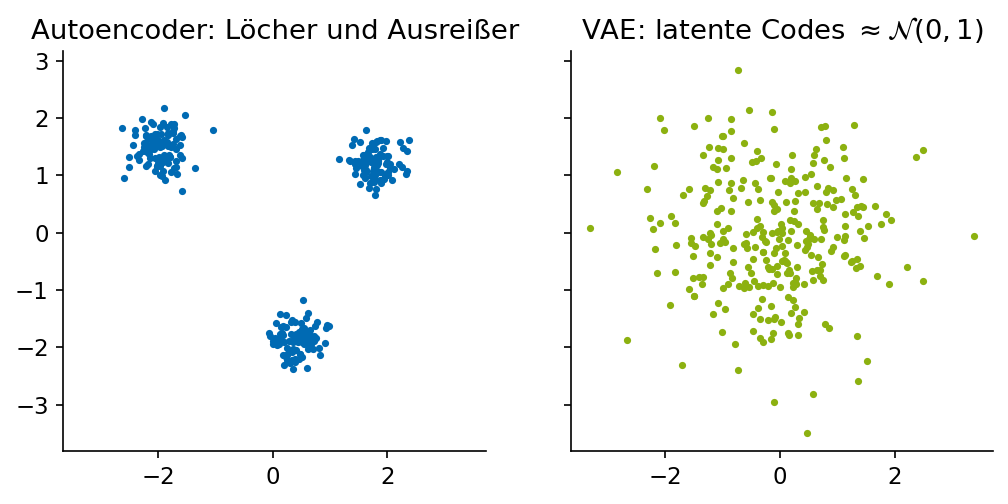
\includegraphics[width=0.62\textwidth]{vl08-latent-300points.png}
  \end{center}

  \note{300 Datenpunkte im latenten Raum eines klassischen Autoencoders: Löcher und
    Ausreißer.
    Frage in den Raum: Was passiert, wenn ich an einer Stelle dekodiere, an der kein
    Datenpunkt liegt? Antwort: Matsch. Genau das wollen wir reparieren --- wir hätten
    gern einen Raum, in dem man \emph{überall} dekodieren kann.}
\end{frame}

\begin{frame}
  \frametitle{Die Idee: Rauschen dazu}

  \begin{center}
    \Large
    Auch $\operatorname{MSE}\bigl(x, \operatorname{dec}(\operatorname{enc}(x) + \varepsilon)\bigr)$
    soll klein sein.
  \end{center}

  \bigskip
  \begin{center}
    \normalsize Der Decoder muss eine ganze \emph{Umgebung} auf $x$ abbilden.
  \end{center}

  \note{Aus jedem Punkt wird eine Wolke. Der latente Raum wird glatt.
    Sofort die Frage stellen, die kommen muss: \emph{Wie geht Backpropagation durch ein
    Sampling?} Antwort: $\varepsilon$ hängt nicht von den Gewichten ab, ist im
    Rückwärtsdurchlauf also eine Konstante --- ganz normale Kettenregel.
    Das ist die Stelle, an der 2025 die meisten Fragen kamen.}
\end{frame}

\begin{frame}
  \frametitle{Drei Punkte, drei Wolken}

  \begin{center}
    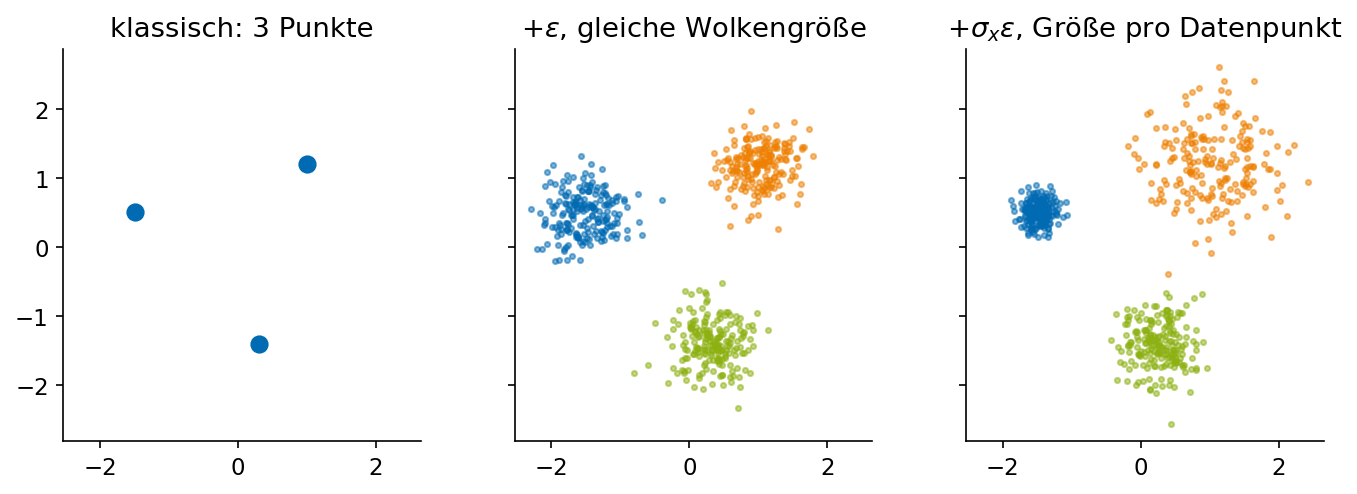
\includegraphics[width=0.78\textwidth]{vl08-latent-3points.png}
  \end{center}

  \note{Links klassisch: drei Punkte. Mitte: mit gleichem Rauschen $+\varepsilon$ ---
    drei gleich große Wolken. Rechts: mit datenabhängigem $\sigma_x$ --- die Wolkengröße
    wird pro Datenpunkt gelernt.
    Das dritte Bild ist der VAE.}
\end{frame}

\begin{frame}
  \frametitle{Der Reparametrisierungstrick}

  \begin{center}
    \Large
    Problem: $\varepsilon \sim \mathcal{N}(0, \sigma_x^2)$ --- $\sigma_x$ hängt an den Gewichten.\\[16pt]
    \Huge $y = \mu_x + \sigma_x\,\varepsilon$, \quad $\varepsilon \sim \mathcal{N}(0,1)$
  \end{center}

  \note{Aus einer Verteilung zu sampeln, deren \emph{Parameter} von den Gewichten
    abhängen, lässt sich nicht ableiten. Nach dem Umschreiben ist $\varepsilon$ wieder
    eine Konstante und $\sigma_x$ ein ganz normaler Ausgang des Encoders, durch den
    Gradienten fließen.
    Das ist die Stelle, an der der VAE steht und fällt --- langsam machen, notfalls an
    der Tafel.}
\end{frame}

\begin{frame}
  \frametitle{VAE-Training}

  \begin{center}
    \Large
    Encoder liefert $2L$ Ausgänge: $\mu_x$ und $\sigma_x$\\[14pt]
    $L_{\text{VAE}} = \operatorname{MSE}(x, \operatorname{dec}(y))
      + D_{KL}\bigl(q(y\mid x)\,\|\,\mathcal{N}(0,1)\bigr)$
  \end{center}

  \note{Ohne KL-Term hat das Training zwei Ausreden: $\sigma_x \to 0$ lernen (dann ist es
    wieder ein klassischer Autoencoder) oder $\mu_x$ explodieren lassen (dann liegen die
    Wolken weit auseinander und der Raum füllt sich nie).
    \textbf{Wichtige Feinheit:} Die beiden $\mathcal{N}(0,1)$ sind \emph{nicht} dasselbe!
    Das erste ist die Rauschquelle, das zweite die Prior-Verteilung, an die sich die
    latenten Verteilungen anschmiegen sollen.
    In der Praxis gibt der Encoder \texttt{logvar} aus, damit kein Ausgang auf positive
    Werte eingeschränkt werden muss.}
\end{frame}

\begin{frame}
  \frametitle{Der KL-Term, geschlossen}

  \begin{center}
    \Huge $D_{KL} = \tfrac12\bigl(\mu^2 + \sigma^2 - 1 - \ln\sigma^2\bigr)$
  \end{center}

  \bigskip
  \begin{center}
    \normalsize Das ist genau der negative ELBO aus Data Science.
  \end{center}

  \note{Für Normalverteilungen gibt es die geschlossene Form --- deshalb ist der Term
    billig.
    Wer nach dem Zusammenhang zu EM fragt: Ein GMM fittet \emph{wenige} Cluster und ordnet
    jeden Punkt einem zu. Der VAE geht umgekehrt vor --- \emph{jeder} Datenpunkt bekommt
    seine eigene Normalverteilung, und der KL-Term sorgt dafür, dass alle zusammen
    ungefähr eine Standardnormalverteilung ergeben.}
\end{frame}

\begin{frame}
  \frametitle{VAE im Bild}

  \begin{center}
    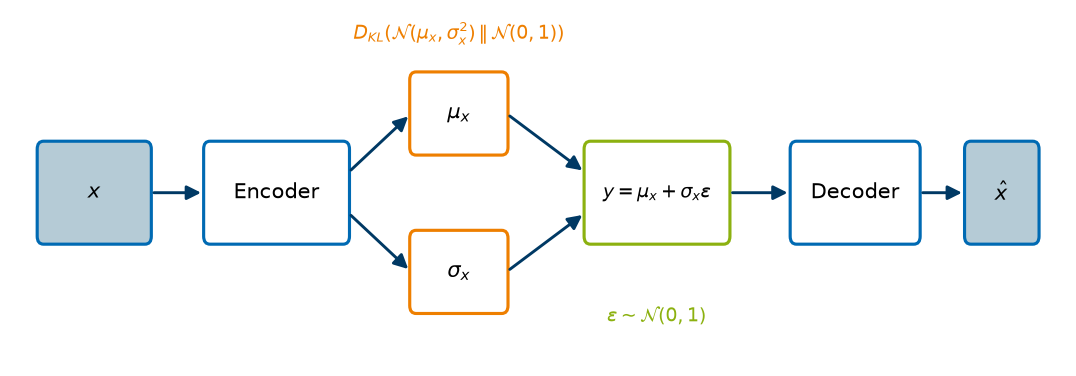
\includegraphics[width=0.66\textwidth]{vl08-vae-schema.png}
  \end{center}

  \note{Recap: Encoder gibt eine Normalverteilung aus, Decoder rekonstruiert aus einer
    Stichprobe, Loss ist Rekonstruktion plus KL zum Prior.
    Und dann kann man \emph{generieren}: $y \sim \mathcal{N}(0,1)$ sampeln und dekodieren.
    VAEs stecken heute noch in Bildgeneratoren --- bei Stable Diffusion findet die
    Diffusion im latenten Raum eines VAE statt.}
\end{frame}

% ------------------------------------------------------------------ word2vec
\begin{frame}
  \frametitle{Dieselbe Idee für Text}

  \begin{center}
    \Large
    Wörter $\longrightarrow$ Vektoren,\\[10pt]
    sodass ähnliche Wörter nah beieinander liegen.
  \end{center}

  \note{One-Hot-Vektoren sind alle gleich weit voneinander entfernt --- ein Autoencoder
    darauf lernt nichts über Bedeutung. Das ist der Punkt, an dem word2vec ansetzt.
    Vorverarbeitung: zählen, Stopwords raus, die häufigsten $N$ (etwa 5000) behalten,
    One-Hot kodieren, und eine Abbildung $\mathbb{R}^N \to \mathbb{R}^K$ mit $K \approx 200$
    suchen.}
\end{frame}

\begin{frame}
  \frametitle{Die Kernidee}

  \begin{center}
    \Large „Die [MASK] frisst ihr Futter am liebsten aus dem goldenen Napf.“
  \end{center}

  \bigskip
  \begin{center}
    \normalsize Die Bedeutung eines Wortes ergibt sich aus seiner Verwendung.
  \end{center}

  \note{Distributional hypothesis. Der Task ist ein Denoising Autoencoder, bei dem das
    Rauschen im \emph{Löschen} eines Wortes besteht --- die Brücke zu letzter Woche
    ausdrücklich schlagen. Und zu Fill-Mask aus VL 3.
    Den Hörsaal raten lassen, was [MASK] ist: Katze, Hündin --- und genau deshalb liegen
    die beiden im latenten Raum nah beieinander.}
\end{frame}

\begin{frame}
  \frametitle{CBOW und Skip-gram}

  \begin{center}
    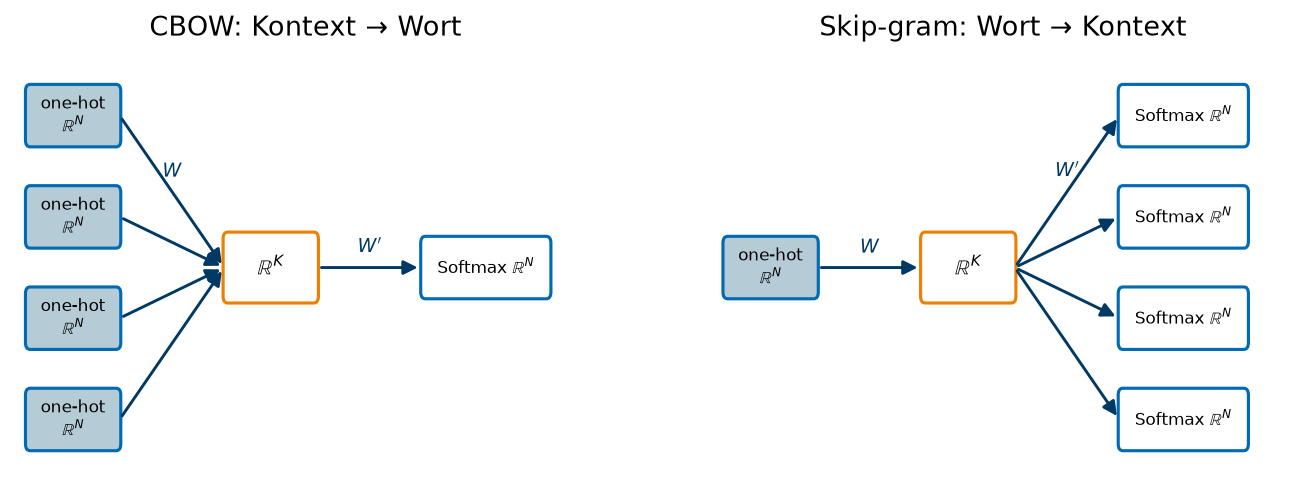
\includegraphics[width=0.72\textwidth]{vl08-cbow-skipgram.png}
  \end{center}

  \note{Zwei Matrizen: $W$ (Encoder, $N \to K$) und $W'$ (Decoder, $K \to N$).
    CBOW: aus $2S$ Kontextwörtern das mittlere vorhersagen. Skip-gram: umgekehrt.
    Loss ist jeweils NLL gegen den One-Hot-Vektor.}
\end{frame}

\begin{frame}
  \frametitle{Wo sind die Wortvektoren?}

  \begin{center}
    \Huge $e(w) = W w$
  \end{center}

  \bigskip
  \begin{center}
    \normalsize Für einen One-Hot-Vektor $w$: einfach die passende \emph{Spalte} von $W$.
  \end{center}

  \note{Das ist die Pointe: Die Matrix $W$ \emph{ist} das Embedding, die
    One-Hot-Multiplikation ist nur ein Lookup. Genau das macht \texttt{nn.Embedding}.
    Fertige Gewichte gibt es bei Gensim oder auf Hugging Face
    (\texttt{word2vec-google-news-300}: $N = 3$ Mio., $K = 300$).
    Klappt schlecht? fastText von Facebook ist Drop-in-Ersatz mit besserem Tokenizer.}
\end{frame}

\begin{frame}
  \frametitle{Wörter? Token!}

  \begin{center}
    \Large
    „Katze isst Maus“ $=$ „Maus isst Katze“?\\[10pt]
    „Schwimmen“ und „schwamm“?\\[10pt]
    „Hund“ und „Tier“?
  \end{center}

  \note{Das sind die Probleme des klassischen Bag-of-Words-Ansatzes, dazu noch die
    bedeutungslosen häufigen Wörter.
    Klassische Antworten: $n$-Gramme, Lemmatisierung, Ontologien, Stopwords.
    Moderne Antwort: nicht Wörter, sondern \emph{Token} als Atome --- Zeichen-$n$-Gramme
    oder gelernte Subwords. „schwimm!“ und „schwimmen“ teilen dann Trigramme.
    Details zur Tokenisierung kommen in VL 10 bei BPE.}
\end{frame}

\begin{frame}
  \frametitle{Anwendung: ähnliche Dokumente finden}

  \begin{center}
    \Large
    Tweets gruppieren, Plagiate finden,\\
    Empfehlungen geben.
  \end{center}

  \note{Der Task, von dem das Kapitel ausgeht: zu $N$ Dokumenten die $k$ ähnlichsten Paare.
    Mit Wortvektoren statt Wortzählungen werden „Hund“ und „Tier“ endlich benachbart.}
\end{frame}

% ------------------------------------------------------------------ Representation Learning
\begin{frame}
  \frametitle{Representation Learning}

  \begin{center}
    \Large
    Features \emph{lernen} statt sie hinzuprogrammieren.
  \end{center}

  \bigskip
  \begin{center}
    \normalsize Ziele: bessere Performance, Generalisierung --- und \emph{Transfer}.
  \end{center}

  \note{Zwei Mechanismen kennen wir schon: Dimensionsreduktion (Autoencoder) und
    nichtlineare neue Features (jede versteckte Schicht tut das).
    Transfer: Ein Encoder, der für Englisch gelernt wurde, taugt auch für Französisch
    etwas.
    Take-Home aus 2025: Alles, was man von Hand bauen kann, kann ein Optimierer
    grundsätzlich auch finden.}
\end{frame}

\begin{frame}
  \frametitle{Handgemachte Features}

  \begin{center}
    \Large
    Spektrogramm einer Audiodatei\\[12pt]
    Kanten und Ecken in einem Bild
  \end{center}

  \bigskip
  \begin{center}
    \normalsize Die automatische Variante davon: CNNs (VL 11).
  \end{center}

  \note{Feature Engineering ist die Handarbeit, Representation Learning die Automatik.
    Das Spektrogramm macht aus einer Waveform ein Bild --- Grundlage für Spracherkennung
    und -synthese.}
\end{frame}

% ------------------------------------------------------------------ Graphen
\begin{frame}
  \frametitle{Ein Satz ist ein Graph}

  \begin{center}
    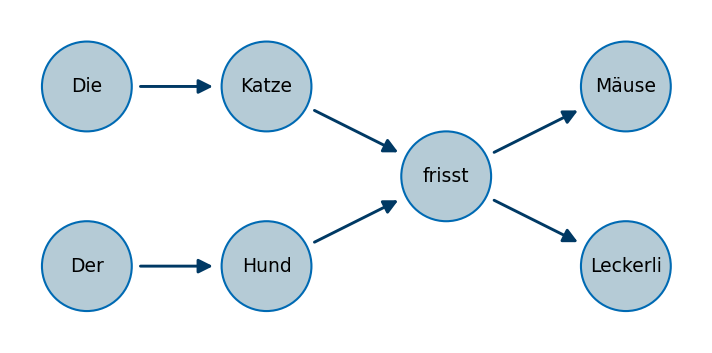
\includegraphics[width=0.72\textwidth]{vl09-sentence-graph.png}
  \end{center}

  \note{Zwei Sätze teilen sich den Knoten „frisst“ --- und erzeugen dadurch Pfade, die
    keine ursprünglichen Sätze sind.
    Das ist die Beobachtung, aus der node2vec entsteht: Wenn Sätze Pfade in einem Graphen
    sind, kann man umgekehrt aus einem Graphen Sätze machen.}
\end{frame}

\begin{frame}
  \frametitle{node2vec}

  \begin{enumerate}\setlength{\itemsep}{10pt}
  \item „Sätze“ durch \emph{Random Walks} auf dem Graphen erzeugen
  \item word2vec-Skip-gram darauf trainieren
  \end{enumerate}

  \bigskip
  \begin{center}
    \normalsize Verstehe einen Knoten durch seinen Kontext.
  \end{center}

  \note{Grover \& Leskovec 2016. Schritt 1 ist teuer, aber parallelisierbar.
    Beispiel, das gut zieht: ein bipartiter Graph Titel $\to$ Genre aus einem
    Netflix-Datensatz --- nach node2vec sucht man im latenten Raum nach ähnlichen Titeln.
    Take-Home: word2vec braucht nur Sätze, also läuft es auf allem, woraus man Sätze
    sampeln kann.
    \emph{Wenn Zeit ist}, die Frage stellen: Wie sähe wav2vec aus? Was sind die „Wörter“,
    was der „Kontext“? 2025 waren das elf Minuten Brainstorming --- dieses Jahr nur, wenn
    die Zeit reicht.}
\end{frame}

\begin{frame}
  \frametitle{Graph Neural Networks: Message Passing}

  \begin{center}
    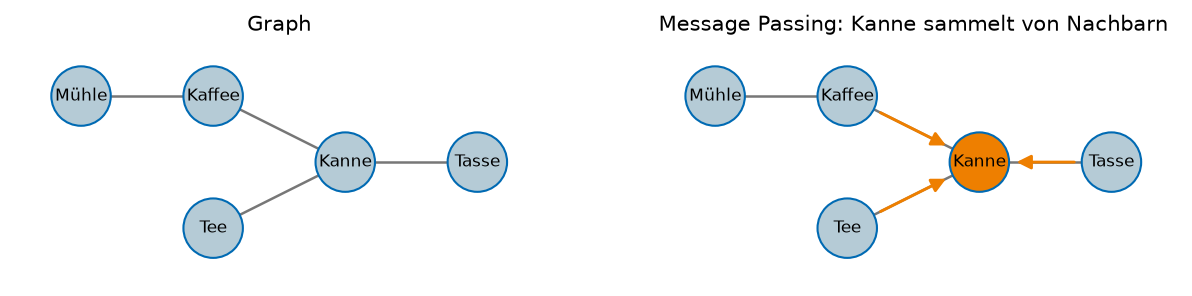
\includegraphics[width=0.66\textwidth]{vl09-message-passing.png}
  \end{center}

  \note{Nur die Idee: Jeder Knoten sammelt Informationen von seinen Nachbarn, mischt sie
    mit seinem eigenen Zustand, und das mehrfach. Nach $k$ Runden weiß ein Knoten etwas
    über seine $k$-Nachbarschaft.
    Die Formel steht als Vertiefung im Skript --- hier nicht vertiefen, das ist Stoff für
    andere Module.}
\end{frame}

\begin{frame}
  \frametitle{Übungsblatt}

  \begin{center}
    \Large Variational Autoencoder auf MNIST.
  \end{center}

  \bigskip
  \begin{center}
    Nächste Woche: Sequenzen --- RNNs und Transformer.
  \end{center}

  \note{Tipp: den KL-Term wirklich addieren (derselbe Fehler wie beim Sparse Autoencoder),
    \texttt{logvar} statt $\sigma$ ausgeben, und am Ende aus $\mathcal{N}(0,1)$ sampeln
    und dekodieren --- erst dann sieht man, ob der latente Raum lückenlos ist.}
\end{frame}

\end{document}

%%% Local Variables:
%%% mode: latex
%%% TeX-master: t
%%% End:
